\documentclass[10pt]{article}

\usepackage{graphicx}
\usepackage{amsmath,amssymb}
\usepackage{gensymb}
\usepackage{mathtools}
\usepackage{etoolbox}
\usepackage{booktabs}
\usepackage{float}
\usepackage{graphicx}
\usepackage{geometry}
\usepackage{multicol}
\usepackage{caption}

\newcommand\mgin{0.5in}
\geometry{
	left=\mgin,
	right=\mgin,
	bottom=\mgin,
	top=\mgin
}

% Set path to import figures from
\graphicspath{{../figures/}}

% Place converted graphics in current directory
\usepackage[outdir=./]{epstopdf}

\newcommand{\plotwidth}{6in}

% Define multicolumn figure-like environment
% from http://tex.stackexchange.com/questions/12262/multicol-and-figures
\newenvironment{mcfig}
	{\par\medskip\noindent\minipage{\linewidth}}
	{\endminipage\par\medskip}

% Define error function for math mode
\newcommand{\erf}{\mbox{erf}}
% Sign function
\newcommand{\sign}{\mbox{sign}}
% Natural numbers
\newcommand\N{\mathbb{N}}
% Real numbers
\newcommand\R{\mathbb{R}}
% Complex numbers
\newcommand\C{\mathbb{C}}
% Curly B for basis
\newcommand\BB{\mathcal{B}}
% Curly R for range (not real numbers)
\newcommand\RR{\mathcal{R}}
% Curly N for null space
\newcommand\NN{\mathcal{N}}
% Norm
\newcommand\norm[1]{\left\lVert #1 \right\rVert}
% Uniform Norm
\newcommand\unorm[1]{\left\lVert #1 \right\rVert_\infty}
% Inner Product
\newcommand\ip[1]{\left\langle #1 \right\rangle}
% Absolute value
\newcommand\abs[1]{\left| #1 \right|}
% Complex Conjugate
\newcommand\conj\overline
% Disable paragraph indentation
\setlength{\parindent}{0pt}
% End of proof
\newcommand\qed{\hfill$\blacksquare$\hspace{0.5in}}

% Number this equation
\newcommand\eqnum{\addtocounter{equation}{1}\tag{\theequation}}


% arara: pdflatex
% arara: pdflatex

\begin{document}

%%fakesection Title
\null

\thispagestyle{empty}
\addtocounter{page}{-1}

\begin{center}
    \begin{sffamily}
	\begin{bfseries}
	    \null
	    \vfill
		\Huge{Survey of Solution Techniques for Linear Systems from Finite Difference Methods in Numerical Radiative Transfer}

	    \vspace{20pt}
	    \LARGE{Advanced Numerical Analysis II} \\
		\LARGE{Final Project} \\
	    \vspace{20pt}
    \begin{Large}
		Oliver Evans \\
		Fred Weiss \\
		Christopher Parker \\
		Emmanuel Arkoh \\[1em]

		Dr. Malena Espa\~nol \\
		Dr. Kevin Kreider \\
		Dr. Curtis Clemons \\
	\vspace{20pt}
	\today
    \end{Large}
	\end{bfseries}
    \end{sffamily}
    \vspace{30pt}

    \null
    \vfill
    \vfill
    \null
\end{center}
\pagebreak


% Increase table cell height (not for header)
\renewcommand{\arraystretch}{1.5}

%\begin{multicols}{2}

\section{Introduction}

We use monochromatic radiative transfer in order to model the light field in an aqueous environment populated by vegetation.
The vegetation (kelp) is modeled by a spatial probability distribution, which we assume to be given.
The two quantities we seek to compute are \textit{radiance} and \textit{irradiance}.
Radiance is the intensity of light in at a particular point in a particular direction, while irradiance is the total light intensity at a point in space, integrated over all angles.
The Radiative Transfer Equation is an integro-partial differential equation for radiance, which has been used primarily in stellar astrophysics; it's application to marine biology is fairly recent.

% CITE MOBLEY HERE


We study various methods for solving the system of linear equations resulting from discretizing the Radiative Transfer Equation.
\subsection{Kelp}
\subsection{Radiative Transfer}
Let $n$ be the number of spatial dimensions for the problem. (i.e., 2 or 3) \\
Let $x \in \RR^n$. \\
Let $\Omega$ be the unit sphere in $\RR^n$.
Let $\omega \in \Omega$ be a unit vector in $\RR^n$. \\
Let $L(x,\omega)$ denote \textit{radiance} - the intensity of light at position $x$ in the direction $\omega$.
Let $I(x)$ denote \textit{irradiance} - the total intensity of light at position $x$.
Let $a(x)$ and $b(x)$ denote the absorption and scattering coefficients respectively of the medium.

Then, the Radiative Transfer Equation is
\begin{equation}
	\label{eq:rte}
	\omega \cdot \nabla_x L(x,\omega) = -(a(x) + b(x)) L(x,\omega)
	+ \int_\Omega \beta(\omega \cdot \omega') L(x,\omega')\, d\omega'
\end{equation}

\section{Discretization}
\begin{figure}[H]
	\centering
	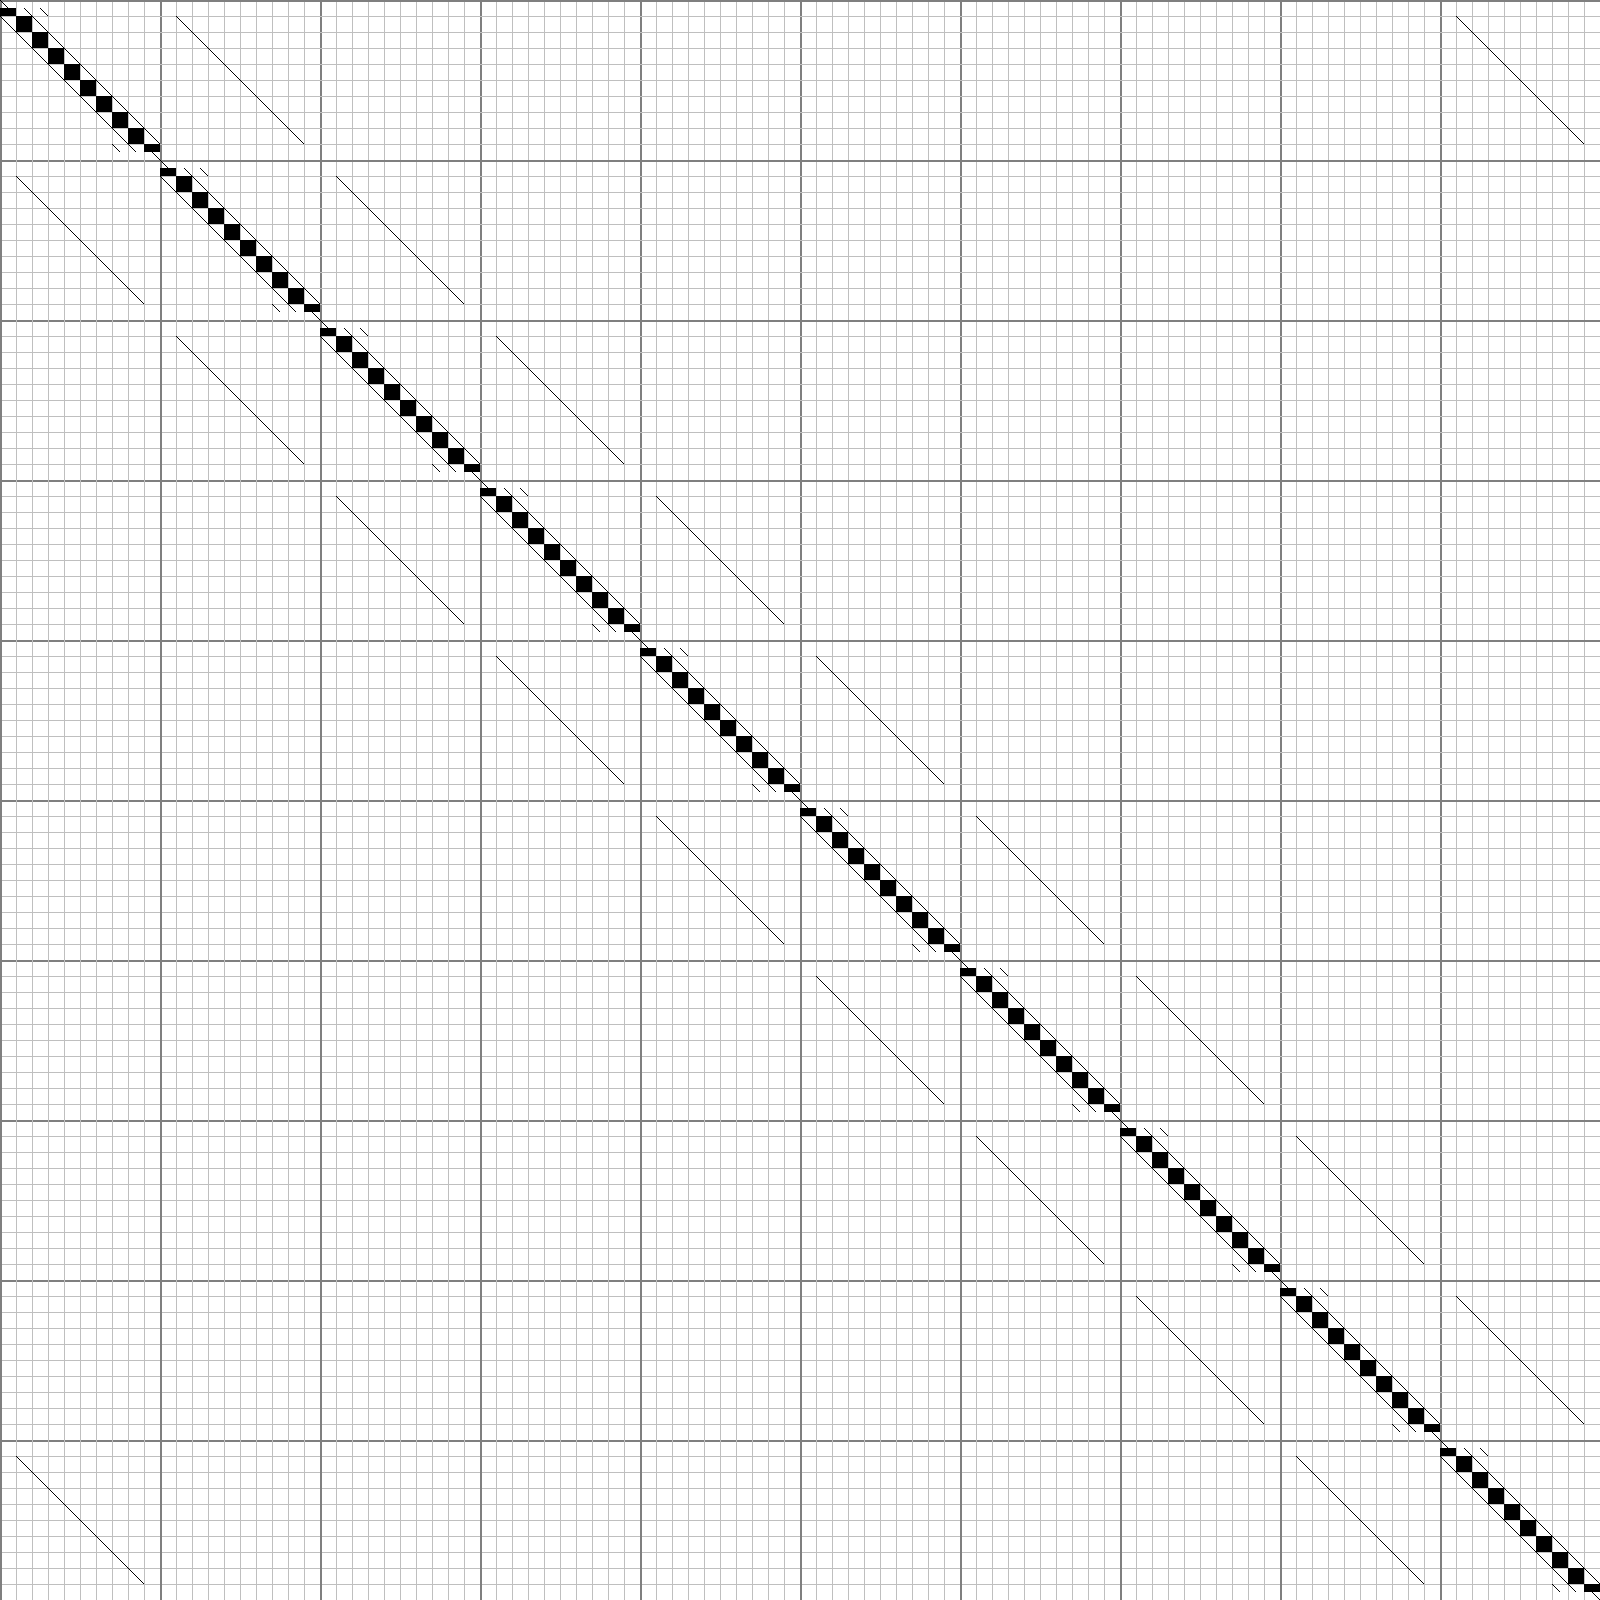
\includegraphics[width=4in]{../img/sparsity/int_kelp1_10x10x16_012.png}
	\caption{Sparsity plot: 10x10x16, ordering 012}
\end{figure}

\begin{figure}[H]
	\centering
	
\includegraphics[width=4in]{../img/sparsity/int_kelp1_10x10x16_210.png}
	\caption{Sparsity plot: 10x10x16, ordering 210}
\end{figure}
\subsection{Sparsity Plots}
\subsection{Matrix Properties}
\subsubsection{Diagonal Dominance}
\subsubsection{Spectral Radius}

\section{Direct Methods}
\subsection{Factorizations}
\subsection{Software Packages}

\section{Stationary Iterative Methods}
\subsection{Fixed-Point Iteration}
\subsection{Convergence and Preconditioning}

\section{Nonstationary Iterative Methods}
\subsection{Krylov Subspace Methods}
\subsection{Convergence and Preconditioning}

\section{Numerical Results}

\section{Conclusions}

%\end{multicols}
\end{document}
